\documentclass[UTF8,a4paper,zihao=-4,fontset=fandol]{ctexart}
% Shared formatting for the course report and research manuscript.
\usepackage[margin=2.2cm,headheight=14pt]{geometry}
\usepackage{amsmath,amssymb,bm,booktabs,tabularx,longtable,array}
\usepackage{graphicx,xcolor,tikz}
\usetikzlibrary{arrows.meta,positioning,calc}
\usepackage{caption,float,placeins}
\usepackage[hidelinks,unicode]{hyperref}
\usepackage{url}
\definecolor{signalblue}{HTML}{205A87}
\definecolor{referenceorange}{HTML}{A95822}
\definecolor{softgray}{HTML}{F0F3F5}
\captionsetup{font=small,labelfont=bf,labelsep=quad}
\renewcommand{\arraystretch}{1.2}
\setlength{\tabcolsep}{4.5pt}
\setlength{\parskip}{0.14em}
\setlength{\emergencystretch}{3em}
\linespread{1.22}
\pagestyle{plain}
\setcounter{tocdepth}{2}
\newcommand{\um}{\,\mu\mathrm{m}}
\newcommand{\ns}{\,\mathrm{ns}}
\newcommand{\mV}{\,\mathrm{mV}}
\newcommand{\fC}{\,\mathrm{fC}}
\newcommand{\V}{\,\mathrm{V}}
\newcommand{\sourcepath}[1]{{\footnotesize\nolinkurl{#1}}}
\graphicspath{{figures/}}
\hypersetup{pdfauthor={},pdfsubject={固定64事件与128响应的r4完整仿真证据；人类课程活动据实待补}}

\newcommand{\EvidenceDate}{2026-10-12 00:34:06 UTC}

\hypersetup{pdftitle={Geant4与TCAD联合仿真的DRAM单粒子读出裕量与冻结预测验证}}
\title{\heiti\Large Geant4与TCAD联合仿真的\\DRAM单粒子读出裕量与冻结预测验证\\[0.5em]\large 基于64独立事件和128配对响应的未校准二维模型}
\author{}\date{\EvidenceDate}
\begin{document}\maketitle
\begin{abstract}基于未校准二维平面访问管与理想电容组成的1T1C模型，建立受约束自然语言输入、Geant4电离沉积到TCAD等效源传递、匹配中性参考及测试前预测冻结的评估流程。统一50~$\Omega$预充版本完成四栅长、两粒子、两个方向下64个独立事件和128个0/1配对响应；训练64响应，域内留出与外推各32响应。在5~mV主阈值下，128个响应中96项正确、20项判据误读、8项临界、4项数值不确定，失败和缺失各为0与0项。域内留出的存储0/1岭回归RMSE分别为0.088294/0.094644~fC（电荷）和0.798415/0.838043~mV（裕量损失）。尺寸外推的存储0/1岭回归RMSE分别为0.068049/0.067155~fC（电荷）和0.519434/0.504929~mV（裕量损失）。14项氧化层case与预定两目标的匹配边界细化通过连续门槛，分类跨界和未选近界状态仍保留数值不确定。工程失败、未知退出码与四项确定性重试全部保全，重试和扩展不增加独立事件数。结论限于固定硅入口、二维等效源、受控准静态初态及所选电磁输运配置；不推断持久位翻转、商业DRAM可靠性或辐射截面。
\end{abstract}
\noindent\textbf{关键词：}DRAM；单粒子效应；匹配参考；数值不确定性；岭回归
\section{引言与相关工作}
动态随机存取存储器（DRAM）依靠存储电容的电荷表示信息。访问晶体管导通后，存储节点与位线发生电荷共享，读出系统依据小幅电压差判断存储状态\cite{keeth2001}。粒子入射在硅中产生电子空穴对，随后发生漂移、扩散和复合；生成电荷、端口收集电荷与存储节点净变化具有不同含义\cite{label1996}。因此，粒子使存储电压变化多少，与给定读出过程能否保持正确差分方向，是两个相关但不能等同的问题。

Geant4与TCAD分别适于描述粒子输运和器件电学响应。陈善强、师立勤已将两类工具用于SRAM单粒子效应评估\cite{chen2011}，因此本研究不将工具耦合本身作为首创贡献。机器学习辅助的TCAD单粒子瞬态回归也已有研究\cite{xu2021}。此外，比较重离子、聚焦X射线和脉冲激光诱导响应的研究指出，生成电荷总量相近并不保证器件瞬态一致，空间分布仍影响响应\cite{ryder2021}。这要求联合模型同时说明源项简化、评价对象与验证边界，而非仅给出软件连接和拟合曲线。

本研究以课程提出的AI辅助多特征尺寸存储器评估任务为背景\cite{course}，聚焦三个问题：第一，有限硅区域内的粒子沉积如何转换为可审计的二维TCAD激励；第二，怎样区分无粒子读出偏移与粒子引起的增量；第三，在源项和无粒子基线已知时，低维回归能否描述不同尺寸、粒子和方向下的连续响应。采用简化1T1C单元保留电荷共享与器件输运，暂不模拟完整阵列、真实感放锁存和恢复。

本文将受约束输入生成、等效源检查、匹配评价、预测冻结和全量验证组织为可追溯的评估链。定量结果以统一R50主版本的64独立事件、128响应为主，历史D1与100 Ω诊断只解释设计演进，不并入主矩阵。独立尺寸留出、外推及氧化层和边界验证均按既定接口接入本次封存证据。模型仍未校准真实工艺，本文讨论条件仿真响应和冻结预测误差，而不推断商业DRAM失效率。

\section{模型与参数传递}
\subsection{1T1C探索模型及其参数含义}
信号单元由二维平面NMOS、存储电容$C_s$和位线电容$C_b$构成。存储节点记为SN，位线为BL；字线驱动访问晶体管，使SN与BL交换电荷。中性参考采用相同几何、网格、物理模型、电容和时序，其SN初始目标为$0.5\V$。参考器件不施加粒子源。该结构保留了读出驱动对器件和电容的共同作用，但中性状态与信号状态不同，匹配参考并不保证消除所有状态相关响应。

硅横截面宽为$L+0.6\um$、深为$1.2\um$，出平面按$1\um$有效厚度归一化。表\ref{tab:paper-parameters}给出主要设定。四种特征尺寸专指访问晶体管栅长；扫描时名义氧化层、掺杂和集总电容保持不变，因此它们不是四代商业工艺节点。文献支持1T1C和电荷共享原理，而表中的具体数值是继承并冻结的探索设定，尚未由器件电学曲线、版图寄生或实际DRAM数据校准。

\begin{table}[htbp]
\centering\small
\caption{R50主模型的主要参数；取值为项目设定，未作工艺校准}
\label{tab:paper-parameters}
\begin{tabularx}{\textwidth}{@{}p{3.2cm}X@{}}
\toprule
参数 & 取值或定义\\
\midrule
栅长$L$、名义栅氧厚度 & $0.18/0.25/0.35/0.45\um$；$5\,\mathrm{nm}$\\
体区、源漏掺杂 & 硼$10^{17}\,\mathrm{cm}^{-3}$；砷高斯峰值$10^{20}\,\mathrm{cm}^{-3}$\\
源漏深度参数 & $0.12\um$处指定$10^{17}\,\mathrm{cm}^{-3}$，横向因子0.4；不等于净掺杂结深\\
栅功函数、温度 & $4.6\,\mathrm{eV}$；$300\,\mathrm{K}$\\
存储、位线电容 & $C_s=10\,\mathrm{fF}$；$C_b=100\,\mathrm{fF}$\\
信号、中性初态 & 信号$0.1/0.9\V$对应存储0/1；中性$0.5\V$\\
预充与字线 & BL目标$0.5\V$；R50预充通路$50\,\Omega$；WL终值$1.8\V$\\
\bottomrule
\end{tabularx}
\end{table}

器件求解耦合泊松方程、电子与空穴连续性方程及外部电路，采用Fermi统计、OldSlotboom带隙变窄、掺杂相关迁移率、高场饱和、法向电场迁移率修正，以及SRH和Auger复合。瞬态采用后向欧拉离散。理想钳位在$0.6\ns$释放，$0.95\ns$核验初态；粒子在$1\ns$入射，$2.8\ns$提取保持阶段指标。BL在$2.8$--$2.9\ns$预充，$3\ns$将预充电阻切至$10^{20}\,\Omega$；WL在$3.05$--$3.10\ns$上升，$4\ns$采样。受控初态使尺寸和位值的比较有共同起点，但不构成真实写入过程的验证。

\subsection{输运几何与等效径迹}
Geant4 10.7.3采用option4电磁构造器和步长限制\cite{g4em}。粒子为$5\,\mathrm{MeV}$的alpha或proton，方向角为$0^\circ/30^\circ$；材料仅含硅和外部真空。硅横截面与TCAD对应，入射点为$(L+0.45,0,0)\um$，方向为$(-\sin\theta,\cos\theta,0)$，$+y$指向硅体内部。有限直径迹长度为
\begin{equation}
\ell=\begin{cases}
1.2\um,&\theta=0^\circ,\\
\min\!\left(\dfrac{1.2}{\cos\theta},\dfrac{L+0.45}{\sin\theta}\right)\um,&\theta=30^\circ.
\end{cases}
\label{eq:paper-length}
\end{equation}
式中$L$以$\mu\mathrm{m}$计。例如$L=0.18\um$、$30^\circ$时从侧边退出，$\ell=1.26\um$；该直径迹不等于散射后的实际输运路程。固定表面入口也意味着本文比较的是约定入射位置，不能推广到整个单元的空间敏感区分布。

\subsection{沉积量到TCAD源项的转换与检查}
设第$j$步总沉积和非电离沉积分别为$E_{{\rm dep},j}$与$E_{{\rm NIEL},j}$，定义
\begin{align}
E_{\rm ion}&=\sum_j\max(0,E_{{\rm dep},j}-E_{{\rm NIEL},j}),\\
Q_{\rm dep}&=q\frac{10^6E_{\rm ion}[\mathrm{MeV}]}{W[\mathrm{eV}]},\qquad
W=3.6\,\mathrm{eV},\quad q=1.602176634\times10^{-19}\,\mathrm{C}.
\label{eq:paper-qdep}
\end{align}
$W$是硅中生成一对电子空穴的平均能量约定\cite{ryder2021}。$Q_{\rm dep}$表示一类载流子的生成电荷尺度，不是产生的净电荷，也不是SN最终损失的电荷。

将总量沿式\eqref{eq:paper-length}的直径迹均匀分配，线电荷密度为$\lambda_{\rm eq}=Q_{\rm dep}/\ell$，横向高斯尺度为$0.03\um$。程序字段\texttt{LET}采用$\mathrm{pC}/\mu\mathrm{m}$，与常用质量阻止本领单位不同。逐步沉积记录用于溯源；实际激励是总量等效源，未忠实传递三维逐步沉积及其时空分布。

对TCAD生成率$G_{\rm ion}$作时空积分，并将二维归一化厚度计入体积元：
\begin{equation}
Q_{\rm src}=q\int\!\!\int_{\Omega}G_{\rm ion}(\mathbf r,t)\,\mathrm dV\,\mathrm dt,
\qquad \frac{|Q_{\rm src}-Q_{\rm dep}|}{Q_{\rm dep}}\leq5\%.
\label{eq:paper-source}
\end{equation}
相对门槛适用于正沉积事件，合法零沉积单独检查近零源项。侧边高斯截断不能通过改小目标沉积量来通过检查。该积分检验转换总量；对等效分布的物理适用性，仍须保留降维近似的限制。

\section{AI辅助流程及评价指标}
\subsection{受约束交互与证据链}
流程如图\ref{fig:paper-workflow}所示。AI辅助编写和审查参数生成、结果提取与证据核验程序；自然语言入口接受约定中文模板，映射到粒子、方向、尺寸和存储位等结构化参数，再检查范围与单位。R50演示支持预览、审计和定位已有证据，实际求解由冻结输入和固定控制器执行。该结果证明受约束请求的参数映射，不能写成任意自然语言生成任意模型或自主开启新求解。

\begin{figure}[htbp]
\centering
% Conceptual workflow, not a measured result or screenshot.
\resizebox{\linewidth}{!}{%
\begin{tikzpicture}[
 block/.style={draw=signalblue,rounded corners=2pt,fill=softgray,
 text width=4.2cm,minimum height=1.5cm,align=center,font=\small},
 arrow/.style={-{Latex[length=2.4mm]},thick,draw=signalblue},
 node distance=0.7cm and 0.6cm]
\node[block] (request) {限定中文请求\\尺寸、粒子、角度\\独立事件数};
\node[block,right=of request] (matrix) {受约束的工况清单\\单位、范围、版本与种子};
\node[block,right=of matrix] (transport) {Geant4 硅内电离沉积\\$E_{\rm ion}\ \rightarrow\ Q_{\rm dep}$\\有限径迹及单位检查};
\node[block,below=of transport] (tcad) {TCAD 器件与电路求解\\等效径迹与受控初态\\读出瞬态与端口检查};
\node[block,left=of tcad] (metric) {匹配中性参考与同位对照\\$D,\ M,\ \Delta Q,\ \Delta M$};
\node[block,left=of metric] (model) {按工况分组的响应拟合\\冻结预测后检验未见响应};
\draw[arrow] (request)--(matrix);
\draw[arrow] (matrix)--(transport);
\draw[arrow] (transport)--(tcad);
\draw[arrow] (tcad)--(metric);
\draw[arrow] (metric)--(model);
\node[below=0.40cm of metric,align=center,font=\small,text width=14.5cm]
 {每一层绑定输入版本、运行记录和来源哈希；科学质量门槛与执行状态分别记录。};
\end{tikzpicture}}

\caption{AI辅助评估流程及证据传递。自然语言映射、粒子事件、TCAD响应和冻结预测具有不同产物；本文只将已归档并通过相应检查的数据作为结果。}
\label{fig:paper-workflow}
\end{figure}

每个响应关联模型版本、粒子事件和输入标识。检查覆盖初态、预充、源项积分、端口电流闭合以及所需匹配关系；求解结束标志不足以证明物理评价可用。确定性重跑保留原失败身份并关联替代归档，不增加独立样本。流程将AI建议、固定规则与求解器结果分开，便于定位错误来源；本文未设人工操作对照组，因此不报告AI带来的效率提升比例。

\subsection{粒子增量与读出参考的分工}
分别用$e$、$c$、$n$表示粒子事件、同条件同存储位无粒子对照和中性参考。在保持阶段$t_h=2.8\ns$，定义
\begin{equation}
\Delta Q=C_s\big[V_{{\rm SN},e}(t_h)-V_{{\rm SN},c}(t_h)\big].
\label{eq:paper-dq}
\end{equation}
$\Delta Q$以fC报告，负值表示存储电容相对对照减少电荷。两种位值对同一方向扰动的敏感性不同，因此不能把全部$\Delta Q$称为正的电荷损失。

对位值$b\in\{0,1\}$，在$t_r=4\ns$定义
\begin{align}
D_e&=V_{{\rm BL},e}(t_r)-V_{{\rm BL},n}(t_r),\\
M_e&=(2b-1)D_e,\qquad
M_c=(2b-1)\big[V_{{\rm BL},c}(t_r)-V_{{\rm BL},n}(t_r)\big],\\
\Delta M&=M_c-M_e.
\label{eq:paper-margin}
\end{align}
$D$、$M$、$\Delta M$以mV报告，$\Delta M>0$表示粒子引起裕量下降。中性参考定义读出差分，位匹配对照提取粒子增量；二者不可互换。同一匹配参考在$\Delta M$中相消，也不意味着可以省略它，因为绝对裕量和判据分类仍取决于参考。

主判据阈值为$\epsilon=5\mV$：$M>\epsilon$为正确方向，$M<-\epsilon$为判据误读，$|M|\leq\epsilon$为临界；另按$2.5/10\mV$检查阈值敏感性。阈值为项目约定，未标定实际感放失调和噪声。数值检查不足以支持边界分类的响应保留“数值不确定”，不能并入正确或误读。本文的误读是固定采样时刻的模型判据，不等同于已锁存的持久位翻转。

\subsection{矩阵设计与独立事件单位}
设计包含4种栅长、2种粒子、2个角度，每工况4个独立事件，共64事件。每个事件分别计算存储0和1，共128个配对响应。训练采用$L=0.18/0.35\um$，含32事件、64响应；$L=0.25\um$为尺寸插值留出，$L=0.45\um$为尺寸外推，各16事件、32响应。训练与测试按尺寸分离，配对位值及同事件的氧化层或数值变体均不增加粒子事件分母。该设计检验特定尺寸变化，不构成对任意能量、入射位置或材料体系的泛化验证。

\section{全矩阵响应与敏感性结果}
\subsection{完整128响应与三阈值统计}
在5~mV主阈值下，128个响应中96项正确、20项判据误读、8项临界、4项数值不确定，失败和缺失各为0与0项。
每个尺寸/粒子/方向/位值分层的预定N保持4，零次明确误读不能推出总体风险为零。表中有效分类已传播近界和细化跨界不确定性，原分类另见完整响应CSV。

\begin{table}[htbp]
\centering\small
\caption{完整128响应在三阈值下的有效状态；失败与缺失不计为正确。}
\label{paper:thresholds}
\begin{tabular}{rrrrrrr}
\toprule
阈值/mV & 正确 & 判据误读 & 临界 & 数值不确定 & 失败 & 缺失\\
\midrule
2.5 & 96 & 27 & 4 & 1 & 0 & 0\\
5 & 96 & 20 & 8 & 4 & 0 & 0\\
10 & 96 & 5 & 26 & 1 & 0 & 0\\
\bottomrule
\end{tabular}

\end{table}

\begin{table}[htbp]
\centering\footnotesize
\caption{按栅长、粒子、位值列出的连续响应范围；每行合并两方向共8响应，未额外增加独立样本。}
\label{paper:ranges}
\begin{tabular}{lclrrr}
\toprule
$L$/\,$\mu$m & 粒子 & 位 & $\Delta Q$/fC & $\Delta M$/mV & $M$/mV\\
\midrule
0.18 & $\alpha$ & 0 & -4.821至-3.560 & -45.514至-33.619 & 71.116至83.011\\
0.18 & $\alpha$ & 1 & -5.412至-3.967 & 37.026至50.550 & -13.213至0.311\\
0.18 & 质子 & 0 & -0.402至-0.164 & -3.784至-1.545 & 39.041至41.281\\
0.18 & 质子 & 1 & -0.436至-0.181 & 1.685至4.066 & 33.270至35.651\\
0.25 & $\alpha$ & 0 & -4.701至-3.732 & -44.357至-35.148 & 72.537至81.746\\
0.25 & $\alpha$ & 1 & -5.166至-4.118 & 38.339至48.114 & -10.880至-1.105\\
0.25 & 质子 & 0 & -0.460至-0.239 & -4.317至-2.241 & 39.631至41.706\\
0.25 & 质子 & 1 & -0.496至-0.257 & 2.391至4.609 & 32.626至34.844\\
0.35 & $\alpha$ & 0 & -4.862至-4.081 & -45.601至-38.220 & 75.376至82.757\\
0.35 & $\alpha$ & 1 & -5.307至-4.459 & 41.259至49.125 & -12.119至-4.253\\
0.35 & 质子 & 0 & -0.456至-0.145 & -4.250至-1.354 & 38.510至41.406\\
0.35 & 质子 & 1 & -0.488至-0.155 & 1.435至4.509 & 32.496至35.571\\
0.45 & $\alpha$ & 0 & -4.834至-3.886 & -45.066至-36.161 & 73.090至81.994\\
0.45 & $\alpha$ & 1 & -5.249至-4.208 & 38.699至48.287 & -11.506至-1.918\\
0.45 & 质子 & 0 & -0.509至-0.229 & -4.716至-2.120 & 39.048至41.645\\
0.45 & 质子 & 1 & -0.544至-0.244 & 2.237至5.000 & 31.781至34.544\\
\bottomrule
\end{tabular}

\end{table}

\begin{figure}[htbp]
\centering
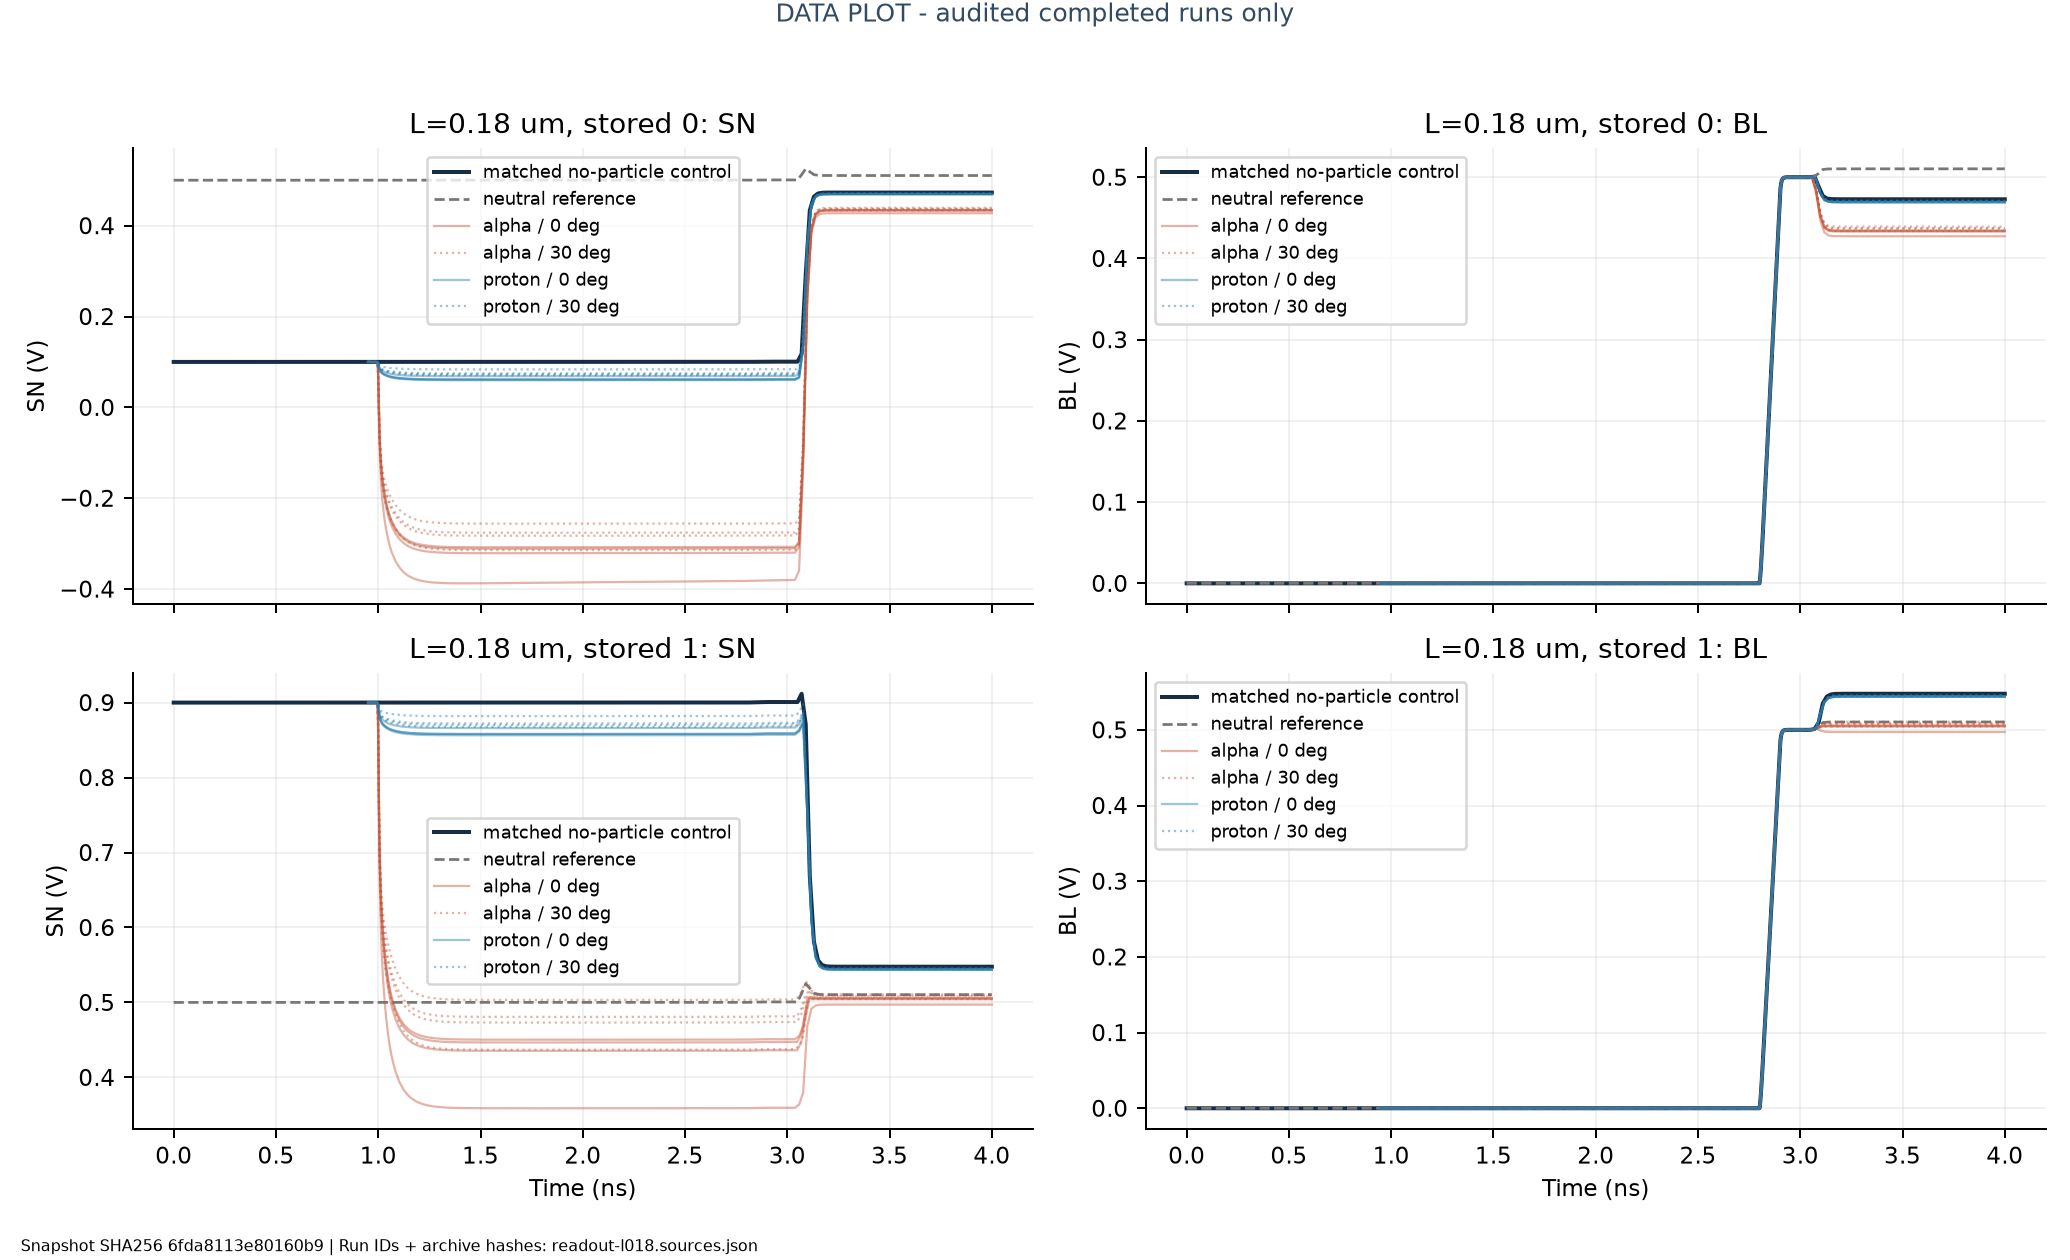
\includegraphics[width=.95\textwidth]{readout-l018.png}
\caption{0.18~$\mu$m的全部事件、同位control与neutral读出曲线；数据来自统一R50快照。}
\label{paper:readout}
\end{figure}

\begin{figure}[htbp]
\centering
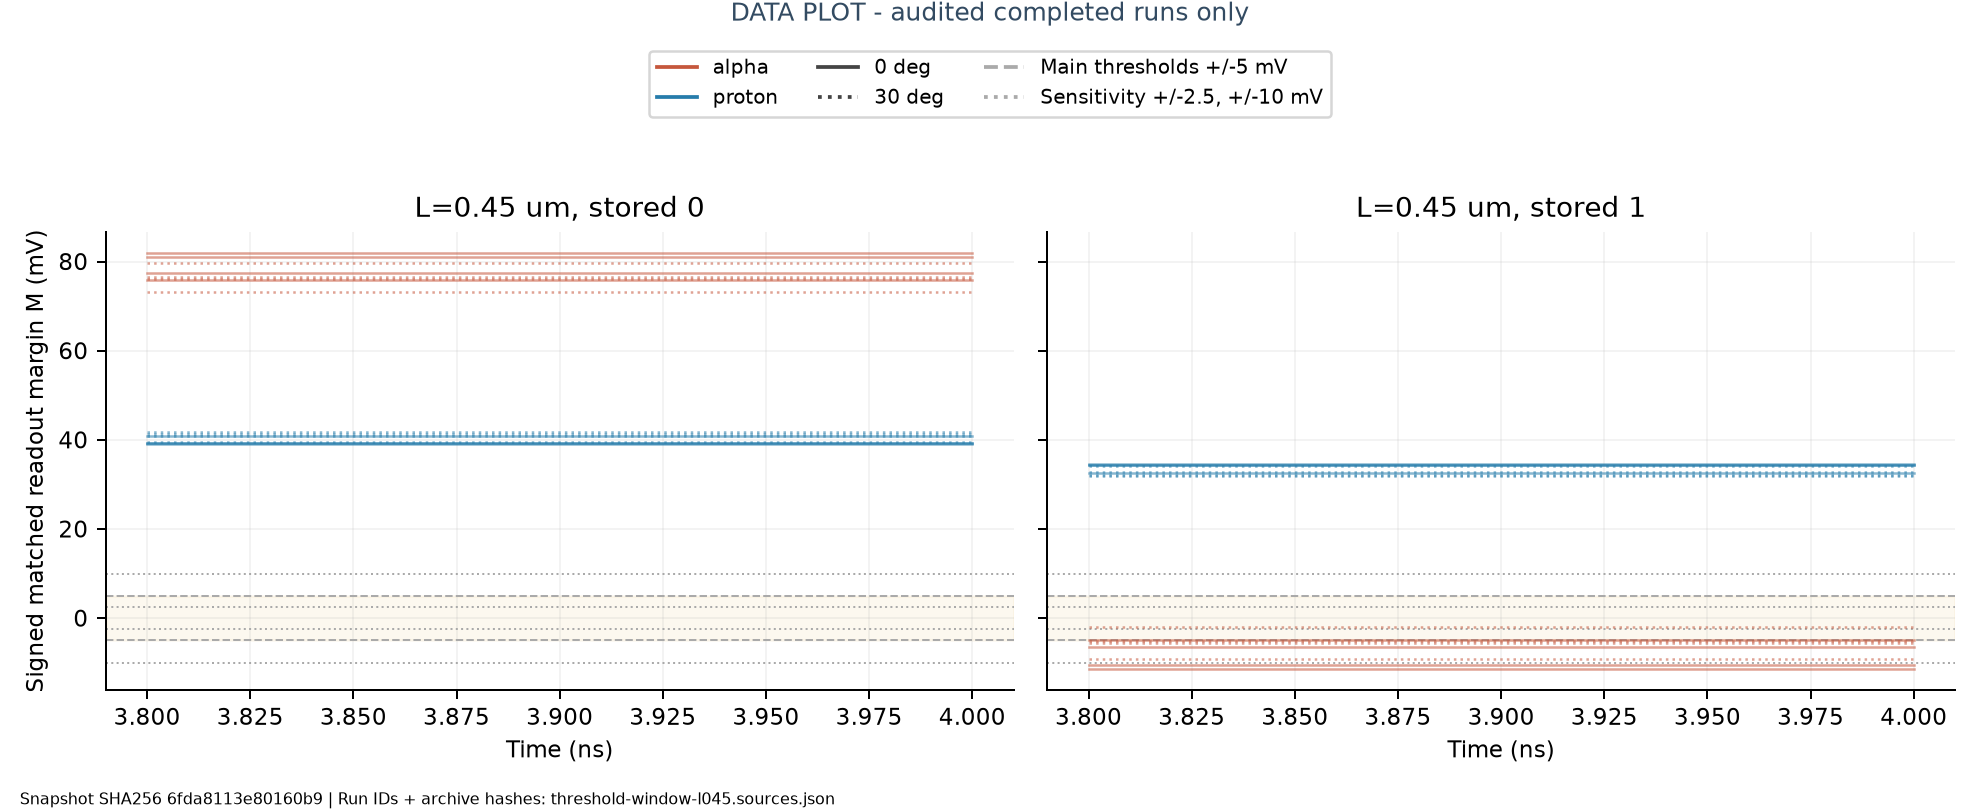
\includegraphics[width=.95\textwidth]{threshold-window-l045.png}
\caption{0.45~$\mu$m外推集合在3.8至4~ns的读出裕量窗口；线条和阈值均来自封存快照。}
\label{paper:window}
\end{figure}
\subsection{原冻结模型的独立留出与外推}
四模型由训练工况LOCO选择，冻结后不再调参。
\begin{table}[htbp]
\centering\small
\caption{八个物理工况折RMSE的算术平均；仅用于训练阶段模型选择。}
\label{paper:cv}
\begin{tabular}{llrrr}
\toprule
位 & 目标 & $\lambda$ & 岭回归RMSE & 均值基准RMSE\\
\midrule
0 & $\Delta Q$/fC & 0.1 & 0.102888 & 2.279967\\
0 & $\Delta M$/mV & 0.1 & 0.955160 & 21.458870\\
1 & $\Delta Q$/fC & 0.1 & 0.112903 & 2.515710\\
1 & $\Delta M$/mV & 0.1 & 1.012491 & 23.383861\\
\bottomrule
\end{tabular}

\end{table}
域内留出的存储0/1岭回归RMSE分别为0.088294/0.094644~fC（电荷）和0.798415/0.838043~mV（裕量损失）。尺寸外推的存储0/1岭回归RMSE分别为0.068049/0.067155~fC（电荷）和0.519434/0.504929~mV（裕量损失）。本次原r4评分与最终连续有效性评分逐项一致。
分类临界或跨界与连续量有效性分别处理；原r4首次评分的原字节副本与最终数值评分均附在证据包。

\begin{table}[htbp]
\centering\footnotesize
\caption{$\Delta Q$的固定预测误差，单位fC。每模型/位/集合计划16响应；缺失和无效显式报告。}
\label{paper:scoreq}
\begin{tabular}{lllrrrrrr}
\toprule
集合 & 位 & 模型 & $n$ & 缺失 & 无效 & MAE & RMSE & 最大误差\\
\midrule
留出 & 0 & 均值基准 & 16 & 0 & 0 & 1.942616 & 1.956036 & 2.416036\\
留出 & 0 & 岭回归 & 16 & 0 & 0 & 0.056607 & 0.088294 & 0.181592\\
留出 & 1 & 均值基准 & 16 & 0 & 0 & 2.140865 & 2.154850 & 2.651122\\
留出 & 1 & 岭回归 & 16 & 0 & 0 & 0.061766 & 0.094644 & 0.198945\\
外推 & 0 & 均值基准 & 16 & 0 & 0 & 2.011262 & 2.025386 & 2.548969\\
外推 & 0 & 岭回归 & 16 & 0 & 0 & 0.052826 & 0.068049 & 0.136393\\
外推 & 1 & 均值基准 & 16 & 0 & 0 & 2.183932 & 2.198297 & 2.733561\\
外推 & 1 & 岭回归 & 16 & 0 & 0 & 0.051740 & 0.067155 & 0.144228\\
\bottomrule
\end{tabular}

\end{table}

\begin{table}[htbp]
\centering\footnotesize
\caption{$\Delta M$的固定预测误差，单位mV。测试没有反向参与选模。}
\label{paper:scorem}
\begin{tabular}{lllrrrrrr}
\toprule
集合 & 位 & 模型 & $n$ & 缺失 & 无效 & MAE & RMSE & 最大误差\\
\midrule
留出 & 0 & 均值基准 & 16 & 0 & 0 & 18.320612 & 18.448022 & 22.860163\\
留出 & 0 & 岭回归 & 16 & 0 & 0 & 0.526964 & 0.798415 & 1.645649\\
留出 & 1 & 均值基准 & 16 & 0 & 0 & 19.936695 & 20.066626 & 24.741705\\
留出 & 1 & 岭回归 & 16 & 0 & 0 & 0.549768 & 0.838043 & 1.765441\\
外推 & 0 & 均值基准 & 16 & 0 & 0 & 18.742144 & 18.867683 & 23.569637\\
外推 & 0 & 岭回归 & 16 & 0 & 0 & 0.404964 & 0.519434 & 1.075289\\
外推 & 1 & 均值基准 & 16 & 0 & 0 & 20.091257 & 20.219896 & 24.915029\\
外推 & 1 & 岭回归 & 16 & 0 & 0 & 0.387723 & 0.504929 & 1.105078\\
\bottomrule
\end{tabular}

\end{table}

\begin{figure}[htbp]
\centering
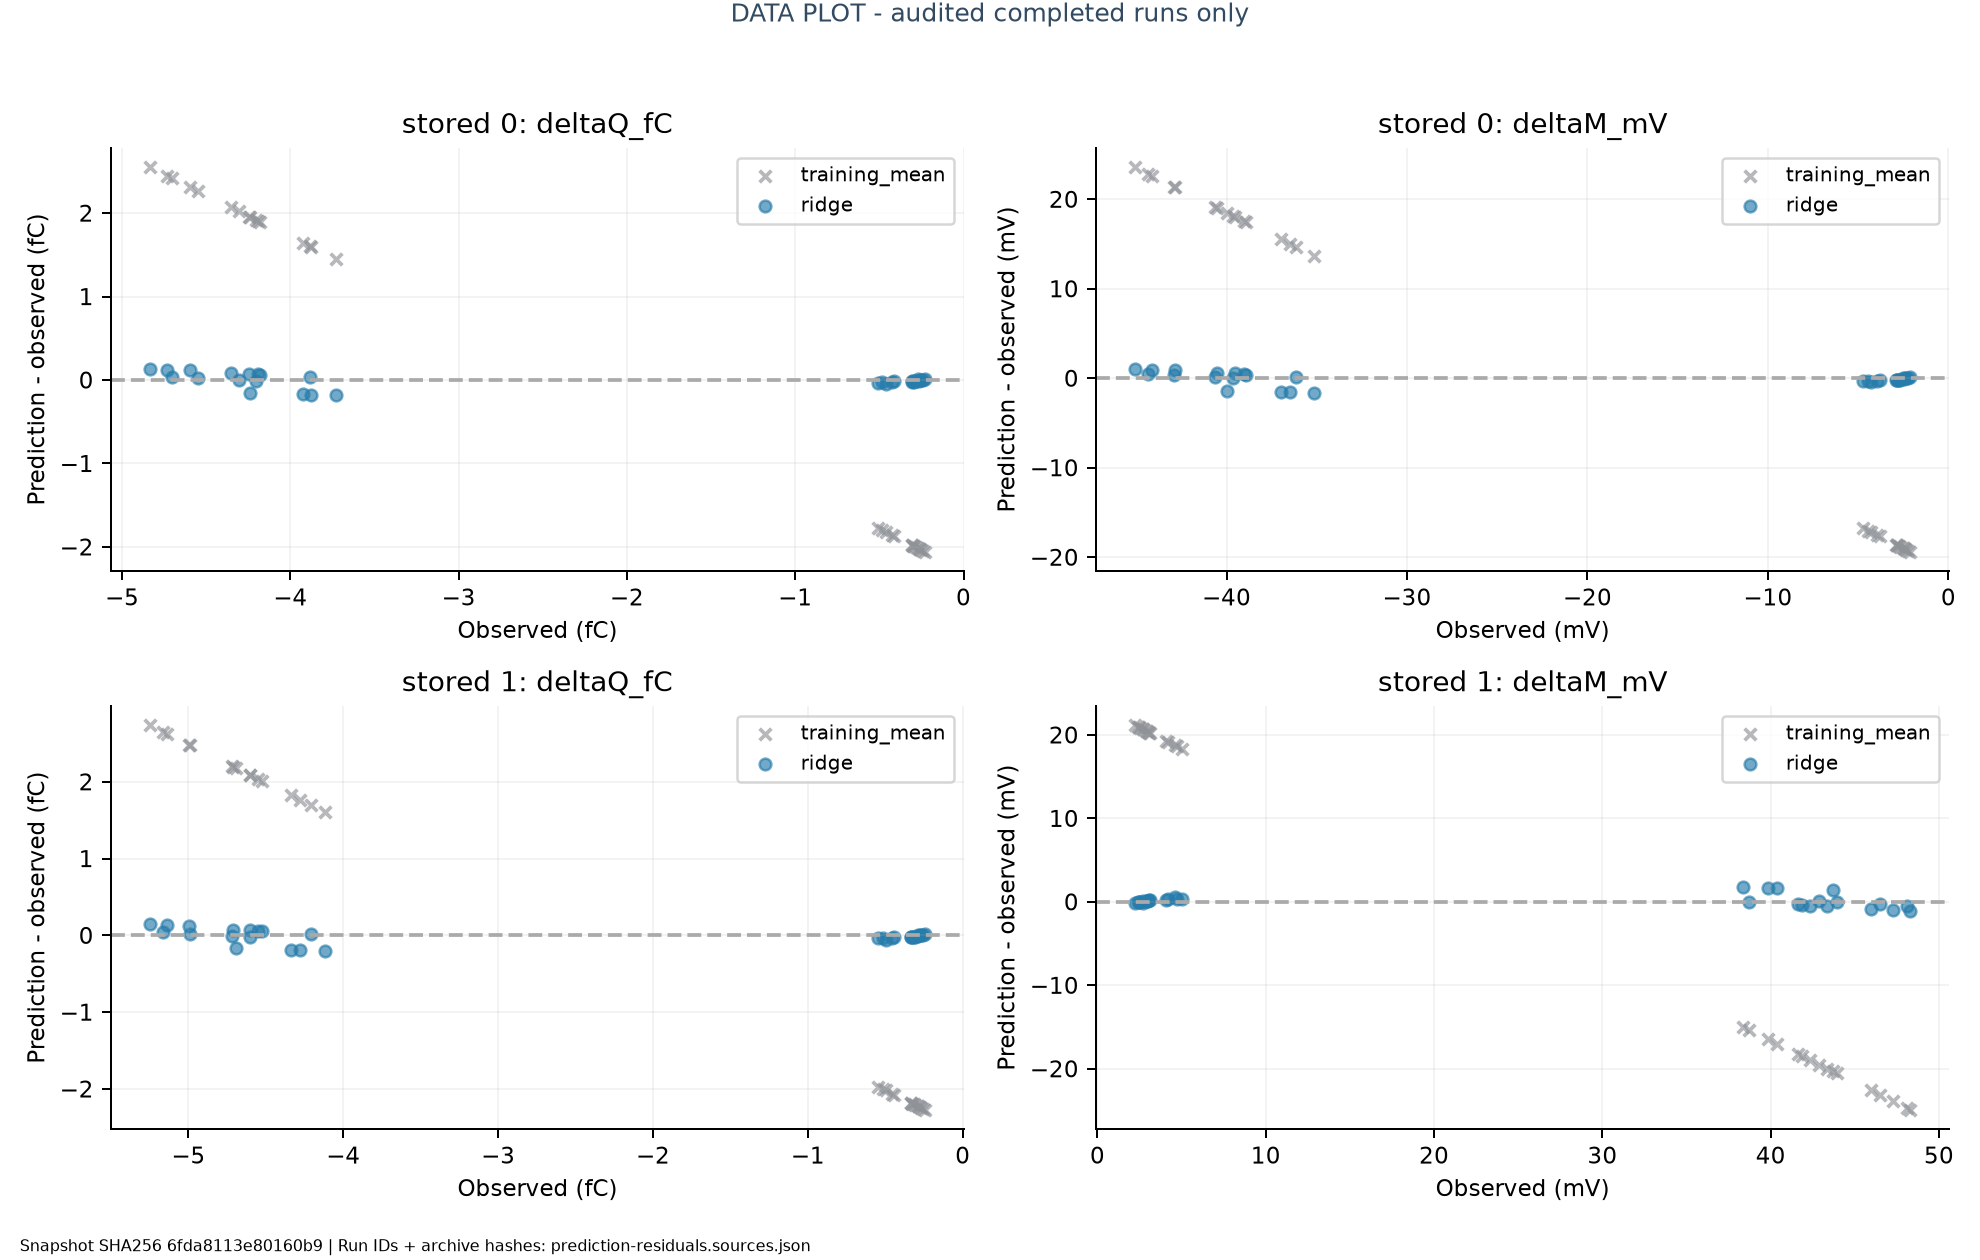
\includegraphics[width=.95\textwidth]{prediction-residuals.png}
\caption{冻结预测减去实际观测的留出/外推残差；训练均值与岭回归均保留。}
\label{paper:residuals}
\end{figure}
\subsection{氧化层敏感性}
在0.25~$\mu$m、垂直入射的固定alpha/质子首个事件上，4/6~nm厚度各建立独立0/1对照、中性参考和事件响应，共14个case。5~nm复用对应四个主响应；含原质子bit0的r3有效alias。每个新厚度实际重建网格，事件三文件字节保持一致。

\begin{table}[htbp]
\centering\footnotesize
\caption{相对于对应5~nm响应的氧化层变化；$\delta(\Delta Q)$和$\delta(\Delta M)$是新厚度减5~nm。}
\label{paper:oxide}
\begin{tabular}{llrrrr}
\toprule
粒子 & 位 & $t_{ox}$/nm & $\delta(\Delta Q)$/fC & $\delta(\Delta M)$/mV & $M$/mV\\
\midrule
$\alpha$ & 0 & 4 & -0.00240 & 0.06772 & 77.8443\\
$\alpha$ & 0 & 6 & -0.00578 & -0.11012 & 78.1679\\
$\alpha$ & 1 & 4 & -0.00464 & -0.06297 & -6.7275\\
$\alpha$ & 1 & 6 & -0.00484 & 0.11256 & -6.7559\\
质子 & 0 & 4 & -0.00022 & 0.00324 & 39.5380\\
质子 & 0 & 6 & -0.00028 & -0.00589 & 39.6928\\
质子 & 1 & 4 & -0.00022 & -0.00377 & 34.7574\\
质子 & 1 & 6 & -0.00027 & 0.00621 & 34.8945\\
\bottomrule
\end{tabular}

\end{table}

\begin{figure}[htbp]
\centering
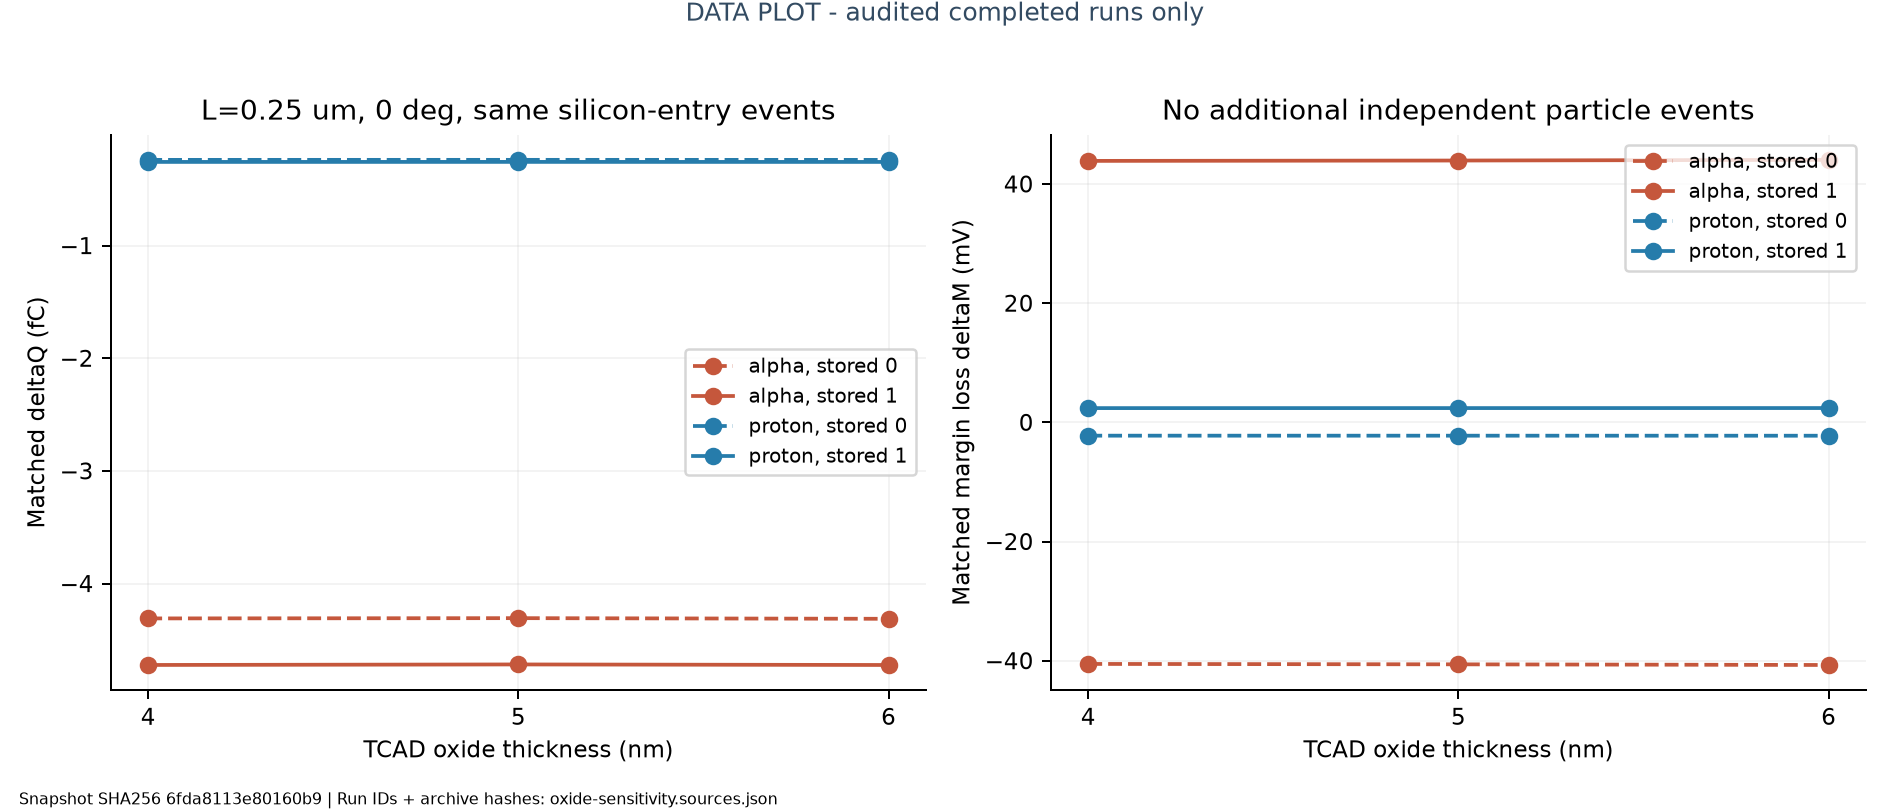
\includegraphics[width=.95\textwidth]{oxide-sensitivity.png}
\caption{4/5/6~nm在固定硅入口事件下的TCAD敏感性；不表示变化材料栈的Geant4输运。}
\label{paper:oxidefig}
\end{figure}
八个新事件响应相对于5~nm的最大绝对变化为0.112560497~mV（裕量损失）和约0.005783687~fC（电荷），分类保持。这些幅度小于预定验收容差0.5~mV和0.01~fC；容差不是统计误差条或已估计的分辨率。每个氧化层响应未再做独立细化和统计校准，故只报告固定入口事件下幅度较小的受控敏感性，不主张零效应、微小效应已可靠分辨或统计显著性。
\subsection{完整矩阵边界细化与原生图}
边界目标由完整128响应到$\pm2.5/5/10$~mV的最小距离排序选取，保持原规则和目标。每目标分别使用半步长与0.7网格的匹配control/neutral/event。四项连续比较均通过，但连续通过不代表类别稳定；5~mV跨界及未选近界响应继续保留不确定性。

\begin{table}[htbp]
\centering\footnotesize
\caption{四个边界比较。最大电压变化包含规定的两侧BL与派生读出量；容差0.5~mV和0.01~fC。}
\label{paper:boundary}
\begin{tabular}{llrrll}
\toprule
事件/位 & 变体 & 最大电压变化/mV & $|\delta\Delta Q|$/fC & 连续门槛 & 不确阈值/mV\\
\midrule
202610304/b1 & 半步长 & 0.032654 & 0.003490 & 通过 & 5\\
202610304/b1 & 0.7网格 & 0.005088 & 0.000009 & 通过 & 无\\
202610313/b1 & 半步长 & 0.025337 & 0.002709 & 通过 & 无\\
202610313/b1 & 0.7网格 & 0.005088 & 0.000006 & 通过 & 无\\
\bottomrule
\end{tabular}

\end{table}

\begin{table}[htbp]
\centering\small
\caption{128响应乘三阈值的384个状态。界外未细化不冒称全部网格独立。}
\label{paper:uncertainty}
\begin{tabular}{lr}
\toprule
阈值响应对状态 & 数量/384\\
\midrule
细化稳定 & 8\\
分类跨界 & 1\\
连续失败 & 0\\
近界待确认 & 5\\
界外未细化 & 370\\
\bottomrule
\end{tabular}

\end{table}

\begin{figure}[htbp]
\centering
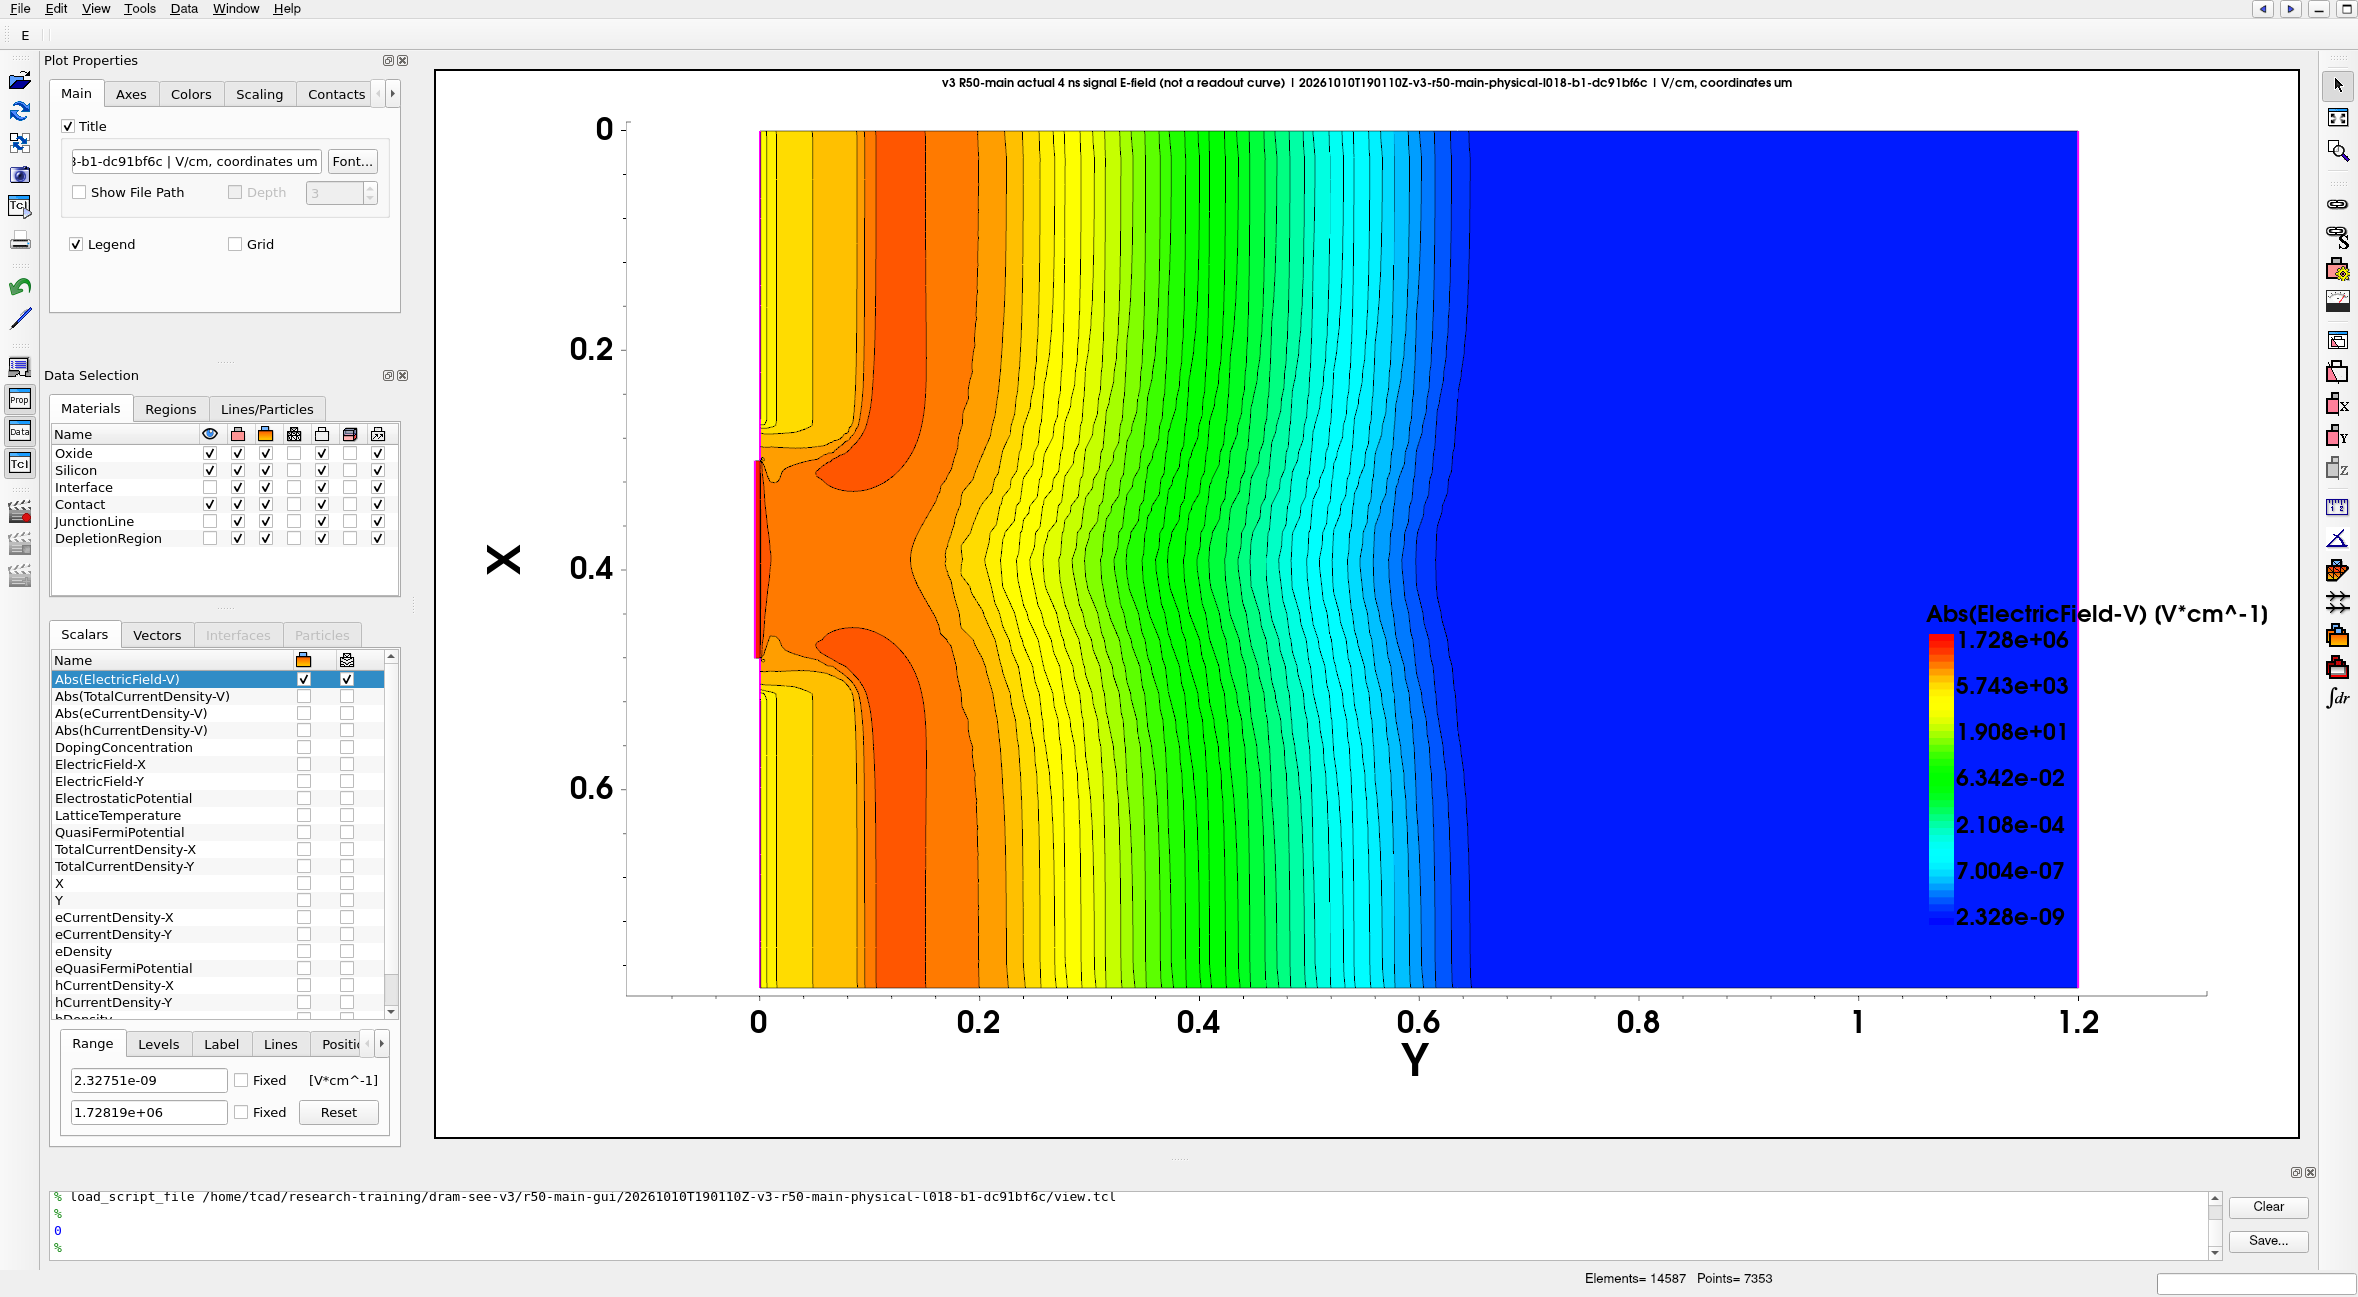
\includegraphics[width=.95\textwidth]{native-physical-window.png}
\caption{真实SVisual owned窗口：0.18~$\mu$m存储1物理参考，4~ns，Abs(ElectricField-V)，V/cm。完整窗口原字节保留并经主代理逐图目视。}
\label{paper:nativephysical}
\end{figure}

\begin{figure}[htbp]
\centering
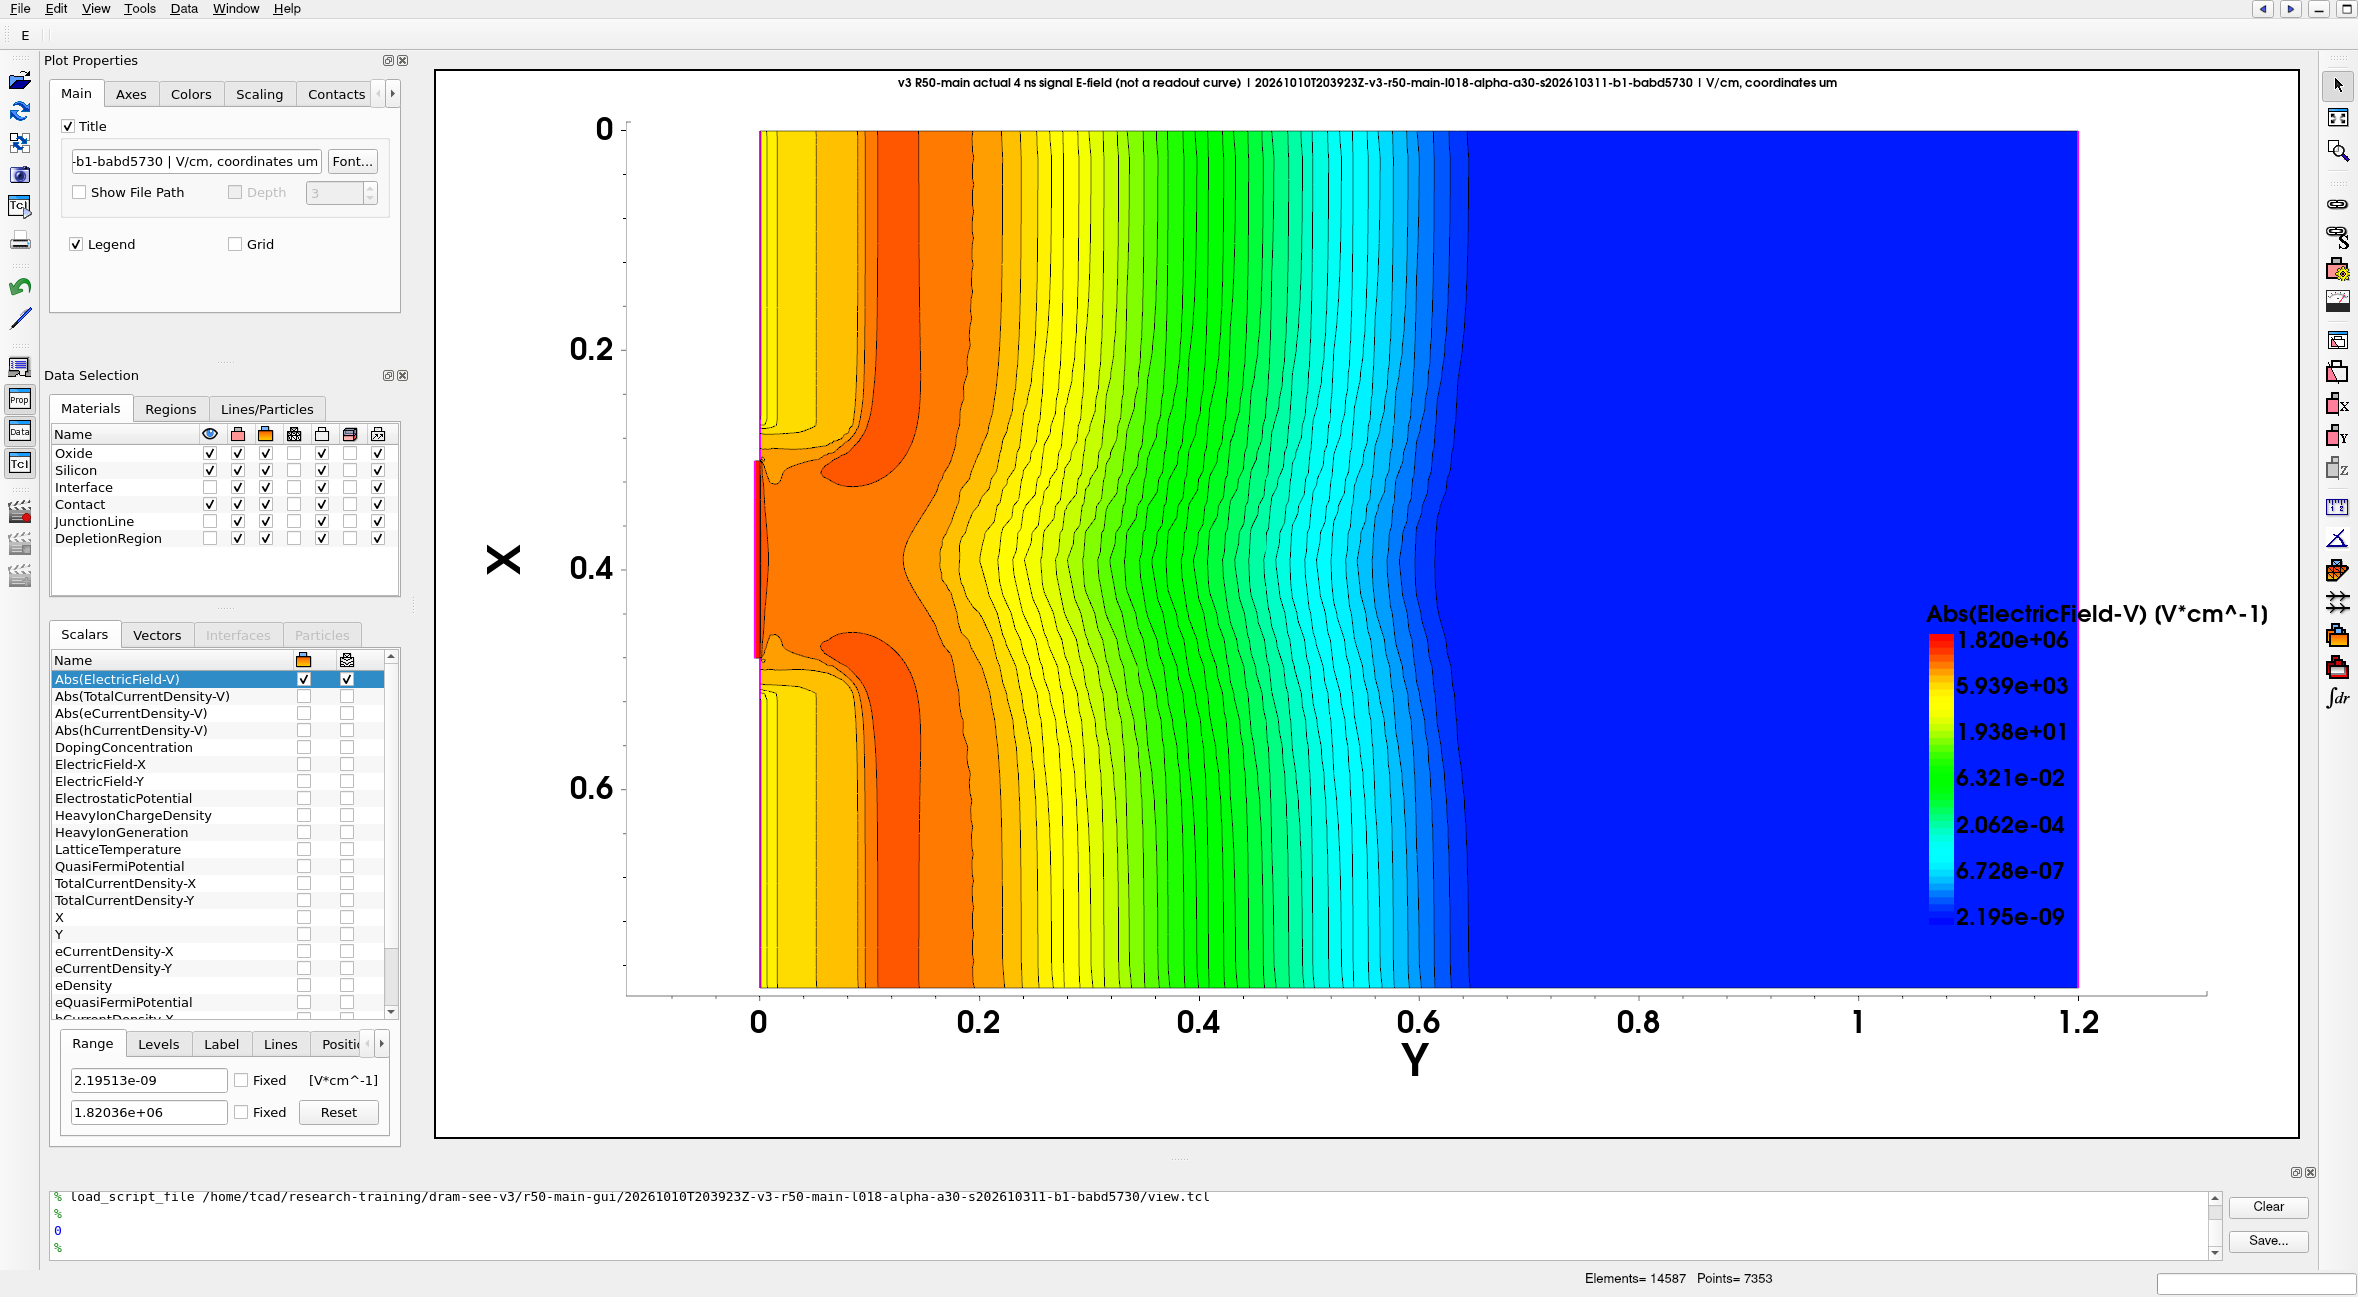
\includegraphics[width=.95\textwidth]{native-event-window.png}
\caption{真实SVisual owned窗口：0.18~$\mu$m、alpha、30°、seed202610311、bit1，4~ns。所示为原窗口，不是数据后处理绘图。}
\label{paper:nativeevent}
\end{figure}
对应1400×1000原生导出右端图例单位后缀存在裁切，已保留并如实记录；本文只展示同组完整owned窗口。真实窗口证明声明的run/变量/时刻，不证明通过Workbench Run按钮调度。
\subsection{失败保全与完整费用}

\begin{table}[htbp]
\centering\small
\caption{四个主线原始工程FAILED及其有效alias。null表示原始退出码未观测，不补写为0。}
\label{paper:failures}
\begin{tabular}{llll}
\toprule
原seed/位 & 有效重试版本 & 原状态 & 原runner退出码\\
\midrule
202610394-b1 & retry-r2 & FAILED & null（未观测）\\
202610353-b0 & retry-r3 & FAILED & null（未观测）\\
202610361-b0 & retry-r3 & FAILED & null（未观测）\\
202610371-b1 & retry-r4 & FAILED & null（未观测）\\
\bottomrule
\end{tabular}

\end{table}
完整历史账本共有7条FAILED记录；表中四项仅是R50主矩阵对应的确定性重试别名。最终逻辑槽失败为0，不表示历史失败为0，全部7条仍在原账本和快照中保留。
唯一全局账本已结算100022.07~s，约27.784~h；含原版本、probe、失败、重试与扩展。当前授权无上限，未结0项、费用缺项0项。该累计求解成本不是学生投入时长或AI效率对照。
\FloatBarrier

\section{预测方法与适用性讨论}
分别对存储0/1的$\Delta Q$和$\Delta M$建立四个岭回归器，特征为
\begin{equation}\mathbf x=(Q_{\rm dep},Q_{\rm dep}/L,Q_{\rm dep}\sin\theta).\end{equation}
八个物理工况留一交叉验证中，每组四次重复及配对位保持同组，标准化仅使用该折训练数据。
候选正则化系数为0、0.01、0.1、1、10，最终参数在测试TCAD首次提交前冻结。
模型是给定Geant4沉积与基线后的条件TCAD响应代理，不代替任意粒子输运。

全量测试扩大了已评价的尺寸范围，却没有校准真实工艺或增加能量、位置、材料栈覆盖。
相同简化模型可能具有共同系统误差，这些误差不会因为训练或测试残差小而消失。
已报告误差须与基准和最差误差一起阅读，不能仅择优列出某个位值或粒子。
低维特征关联不能唯一证明微观收集机制。

存储状态由理想钳位和准静态初态建立，未验证真实写入能力；二维1T1C、固定集总电容和
总量等效直径迹不代表真实立体存储器及三维敏感体积。所选电磁option4的质子结果不包含已验证的
核反应次级粒子效应。4/6 nm结果只是固定硅入口事件下TCAD敏感性，不是完整材料栈输运重算。

连续门槛、判据分类和持久位翻转是不同对象。采样时刻的临界与跨界不能自动解释为商业SEU，
每层N=4也不能支持高精度稀有失效概率。数值细化通过的响应和界外未细化的响应均在完整状态表中区分。
确定性工程重试保留原失败及未知退出码，只恢复原逻辑槽。

AI协助脚本、核验和文稿，固定程序执行数值过程。本研究未设置人工操作对照，因此没有AI加速率结论。
学生与教师活动不是本文软件证据的推论，课程实际审核和答辩保留待完成。

\section{结论}
在5~mV主阈值下，128个响应中96项正确、20项判据误读、8项临界、4项数值不确定，失败和缺失各为0与0项。域内留出的存储0/1岭回归RMSE分别为0.088294/0.094644~fC（电荷）和0.798415/0.838043~mV（裕量损失）。尺寸外推的存储0/1岭回归RMSE分别为0.068049/0.067155~fC（电荷）和0.519434/0.504929~mV（裕量损失）。
本次完成了限定自然语言映射、真实事件到器件源项传递、匹配参考定义、统一主矩阵、预测前冻结、独立留出/外推评分与受控扩展的一致证据链。原科学门槛、样本分母和全部失败保持不变。边界验证显示连续量稳定与分类稳定需要分别报告，不能以一次连续门槛通过清除全部数值不确定。

下一步器件研究需用具有出处的工艺和电学数据校准结构、实际写入、保持、感放及恢复，扩展能量、位置与统计规模。课程方面已形成可编辑报告、研究稿、PPT与只读演示材料；真实学生贡献、教师审核、试讲、答辩和考核由参与者完成并据实留证。

\FloatBarrier\bibliographystyle{unsrt}\bibliography{references}
\clearpage\appendix
\section{证据来源与复现边界}
本稿的输入、数据图、原生图及数值表均由同一r4交付快照绑定，完整文件级索引见
\sourcepath{reports/final-r4/sources.json}与\sourcepath{reports/final-r4/evidence-index.csv}。
原r4评分和扩展数值状态下的最终评分分别保留，模型和64条预测未重新拟合或修改。
原FAILED、未知退出码、四alias以及累计成本由快照原账本提供。
此文稿没有重启任何求解，也没有把程序审计替代实际学生和教师活动。
快照中的采集时PENDING标签保持不变，后续完整机器、统计和逐图目视验收见
\sourcepath{data/delivery-root-acceptance.json}及两份visual-review记录。
\par\medskip\noindent
\begin{tabular}{lp{0.62\textwidth}}
\toprule
证据类别 & 本包入口\\
\midrule
完整128槽及数值状态 & \sourcepath{data/snapshot/responses.csv}\\
真实case owner与四alias & \sourcepath{data/snapshot/response-sources.json}\\
原FAILED和费用 & \sourcepath{data/snapshot/ledger-snapshot.json}\\
原r4固定模型评分 & \sourcepath{data/snapshot/original-r4-prediction-scores.json}\\
最终数值证据评分 & \sourcepath{data/snapshot/final-numerical-prediction-scores.json}\\
原生PNG真实目视 & \sourcepath{data/native-visual-review.json}\\
全部来源与哈希 & \sourcepath{sources.json}\\
\bottomrule
\end{tabular}

\end{document}
